\begin{figure}[H]
    \caption{Estados del nodo de marcador mediante planos}
    \centering
    \setlength{\tabcolsep}{0pt}
    \renewcommand{\arraystretch}{1.2}
    \begin{tabular}{
        |>{\centering\arraybackslash}m{(\textwidth - 4\arrayrulewidth) / 3}
        |>{\centering\arraybackslash}m{(\textwidth - 4\arrayrulewidth) / 3}
        |>{\centering\arraybackslash}m{(\textwidth - 4\arrayrulewidth) / 3}|
    }
        \hline

        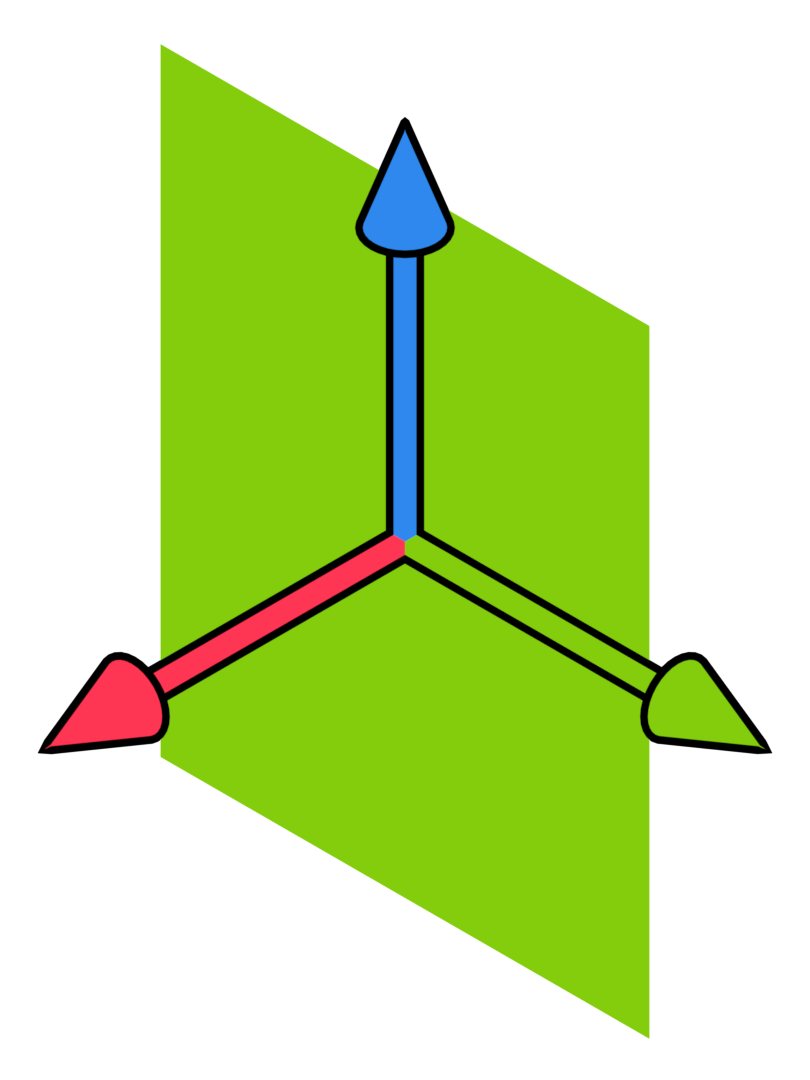
\includegraphics[width=(\textwidth - 4\arrayrulewidth) / 3]
        {assets/figures/second_phase/node/img_node_plane_green.png} &
            
\includegraphics[width=(\textwidth - 4\arrayrulewidth) / 3]
        {assets/figures/second_phase/node/img_node_plane_yellow.png} &
                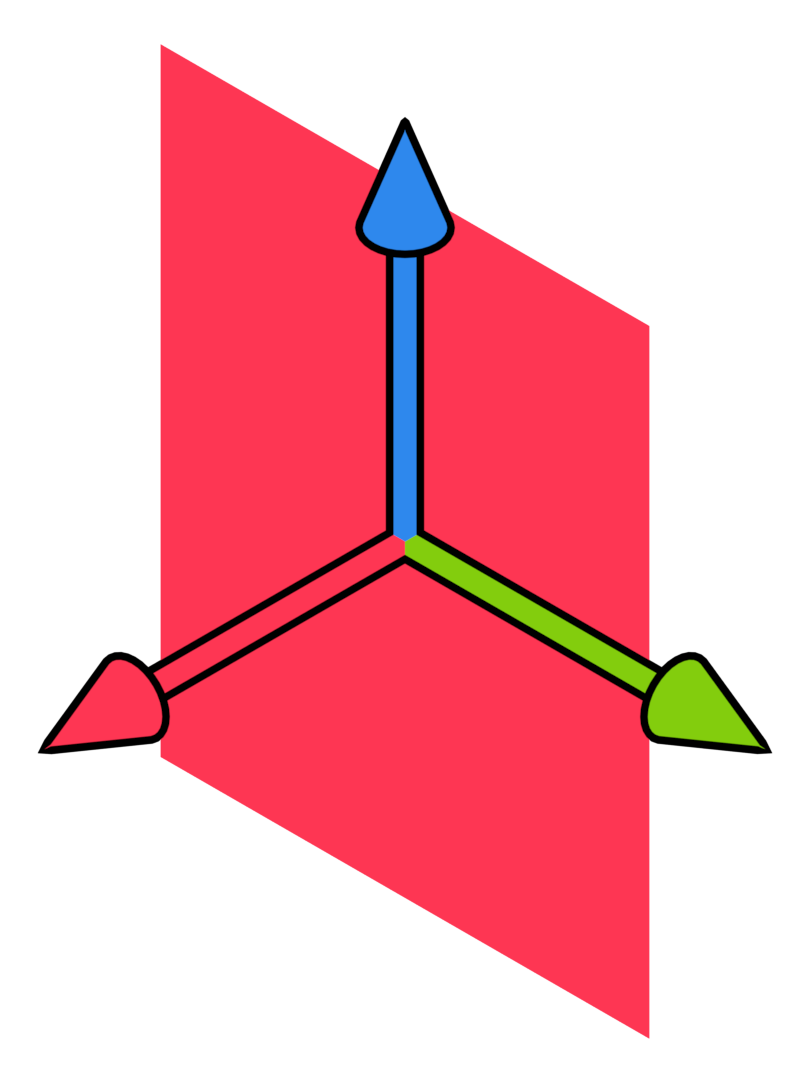
\includegraphics[width=(\textwidth - 4\arrayrulewidth) / 3]
        {assets/figures/second_phase/node/img_node_plane_red.png} \\

        \rule{0pt}{0.8cm}\small Seguimiento activo del marcador &
            \rule{0pt}{0.8cm}\small Pérdida temporal del seguimiento &
                \rule{0pt}{0.8cm}\small Pérdida total del seguimiento \\

        \hline
    \end{tabular}
    \label{fig:node_plane}
\end{figure}
\fixvspace{0}